\documentclass{article}
\usepackage[margin=1.5in]{geometry}
\usepackage{float}
\usepackage{graphicx}
\usepackage{tikz}
\usepackage{pgfplots}
\usepackage{amsmath}
\usepackage{nameref}
\usepackage{siunitx}
\usepackage[utf8]{inputenc}

\newcommand{\cmmnt}[1]{\ignorespaces}
\pgfplotsset{compat=1.13}

\begin{document}

\title{Localization for FRC \\
  \large{A Term Report}
  }
\author{Jinan (Dorothy) Hu, Peter Mitrano, Kacper Puczydlowski, Nicolette Vere}

\maketitle{}

\section{Introduction}

Knowing the position and orientation of a mobile robot is critical to many tasks. For robots designed for high-speed gameplay, knowing the position and orientation allows the robot to perform complex autonomous behaviors such as shooting and retrieving game objects. In this report, we describe a system for determining the pose $(x, y, \theta)$ of a mobile robot in a cluttered environment. The environment we are interested in is the FIRST Robotics Competition (FRC). FRC is a challenging environment because the robots make rapid and aggressive maneuvers by human drivers for part of the time, and at other times are under complete autonomy. A successful localization system for FRC must handle up to six robots, occlusion from the playing field elements, unpredictable lighting, and frequent impacts. Our research suggests that there are at least five appropriate methods for localization: cameras and tags, radio and ultrasonic beacons, optical flow, and dead reckoning with encoders, and dead reckoning with an IMU. All of these methods have seen success in robot localization.

This report begins with a review of existing literature on indoor localization for mobile robots in the \nameref{related_work} section. The strengths and weaknesses of these existing methods are described in the \nameref{methods} section. The \nameref{experiments} section contains information on experiments we conducted. The \nameref{specs} section provides a complete description of our design criteria, and system specifications. The \nameref{conclusion} section details our plan moving forward.

\section{Related Work} \label{related_work}

Robot localization has been studied for decades. Overall, the problem of localizing a mobile robot can be viewed as accurately measure the absolute distance to known landmarks, or by measuring the changes in position over time. We will henceforth refer to these two ideas as global and local pose estimation. Some of the high level techniques for robot localization are: measuring range at various points around the robot and matching these readings to a map, measuring time of flight or difference of time of arrival to calculate distance to known locations, recognizing landmarks in some modality and computing pose relative to those landmarks, and measuring changes in pose and accumulating these changes over time. There are different sensors that can be used for each of these techniques, such as laser range finders, ultrasonic, cameras, inertial measurement units (IMU), encoders, radio, visible light, and human-audible sound. Although there are a tremendous number of possible methods for robot localization, there are a few which have received the most attention and shown the most success. These include:
\begin{itemize}
    \item Lidar mapping
    \item Ultrasonic mapping
    \item IMU and Encoders fusion
    \item Infrared or Radio and Ultrasonic beacons
    \item cameras with visually identifiable tags
    \item Optical flow mice and cameras
    \item Stereo vision and depth cameras
\end{itemize}

In our research, we learned how these seven techniques work and found descriptions and implementations in order to evaluate them. These descriptions and implementations are described in this section with the purpose of demonstrating a thorough literature review and of providing background information to the reader.

An inertial measurement unit (IMU) is a sensor reporting the forces acting upon an object, the angular rates of change, and surrounding magnetic field. The device typically comprises an accelerometer, gyroscope, and magnetometer which sense the above data respectively. These devices function by detecting Coriolis forces, inertial forces acting in the direction of motion relative to a rotating reference frame. These forces are proportional to the magnitude of the acceleration. These forces may be detected by a simple strain gauge mechanism or object vibrating at a know frequency ( the rate of change of vibration frequency is detected) \cite{barshan_199354}. The premise behind position sensing using this device involves integrating the data with respect to time to calculate position and orientation. This approach was first used in aeronautics to estimate projectile attitude, orientation, and position \cite{agard_1989}. High cost IMU's have been used historically for defense and transportation systems; the quality of the sensor is high and the data is reliable in these applications. An inertial navigation system (INS) often comprises multiple accelerometers, gyroscopes, and magnetometers to estimate orientation and position. Their performance is increased by referencing, or filtering, one sensor to estimate the error from another. Simple double integration of a filtered system using expensive sensors is often sufficient for position tracking applications like ballistics or missile tracking \cite{barshan_199354}.

In cost-sensitive systems, this methodology is subject to high error rates from accumulation. Because of integration of accelerometer data, the velocity error term grows linearly and position error quadratically. This introduces a need for filtering, sensor fusion, and optimization based approaches.

	Rarely in mobile applications are IMUs the primary position sensor. Odometers and encoders offer relative position sensing because they measure change between distances, but must be provided with a frame of reference. Most odometry-based sensors are updated at a high-frequency, but are subject to high error rates from gear inefficiencies, wheel slippage during normal rotation, and irregularities in data processing \cite{linchevski_addressing_2007}. Complementary filtering, or using multiple, weighted sources of data, is used to obtain an position estimate. Linear quadratic estimation can be used to estimate the position of a object; however, this technique is relatively complex. The algorithm makes a prediction about the current position, taking into account error from the previous measurements. Once the current data is available, the algorithm uses it to correct the parameters it used to make the estimation, provided the data is of high certainty. Known as a Kalman filter, this process uses a known model of the system and assumes errors in the sensors to smoothen the data. Systems can leverage data from a range sensor \cite{teslic_ekf_2011} or indoor positioning systems that use radio frequency signals \cite{marquez_uwb_2017}.

	Cameras, radio beacons, GPS, and similar landmark-based technologies offer global position sensing and have lower accumulated error than local systems discussed above. However, update frequencies are comparatively low, leading to false predictions or periods of unknown position. To compensate for this phenomenon, systems can leverage data streams with higher update frequencies to interpolate between frames. Forster \textit{et al.} describe a visual-inertial navigation system that uses accelerometer and gyroscope data streamed at a high frequency to estimate a pose trajectory between select frames from the camera. Known as keyframes, these camera data are selected to minimize computational requirements while minimizing feature loss. Often, a parallel thread selects appropriate frames. Then, the IMU data are processed into a relative motion constraint. Effectively, this yields a trajectory of position and orientation between camera updates \cite{forster_CDS_15}.

    If the rate at which the position must be updated is lower than the update rate of the data, many values can be processed and used to calculate an approximation within a given time window. Known as preintegration, this technique, instead of filtering the data, combines many data points into a single trajectory estimate. Then, it transforms the data into the navigation frame, allowing for a smoother approximation of system position. This was beneficial in cases where global position data was unavailable for extended periods of time and decreased the computational load of the localization thread \cite{lupton_vian_2012}. Systems like this are effective because camera data is used to correct IMU data on-line when data is available and rarely fails to update the pose estimate between frames. The above work describes an overall CPU time of about 10ms for data processing and real-time execution, although the system update frequency is unknown.

    Leveraging preintegration, systems expanded sensor fusion frameworks with probabilistic terms and models of relationships between sensors. One such approach used a factor-graph to represent system state variables as nodes on a tree and the functional relationship between them as factors (edges). Instead of updating the state each time new data is available, the factor tree updates relevant state variables add into account an error term \cite{indelman_ifns_2013}. A key aspect of this system relies on frame transformations between sensor data happening at a low level. This takes workload off of the main CPU by utilizing FPGAs or other processors to monitor and process odometry or IMU data \cite{li_gyro_2017}. Implementations of such systems claim reduced computational load and similar performance to ORB-SLAM and other modern navigation systems.

\begin{figure}[H]
  \centering
  \scalebox{.4}{
  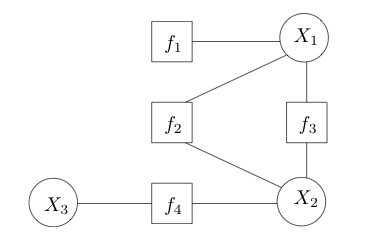
\includegraphics[width=1\linewidth]{./images/Factorgraph.jpg}}
  \label{fig:ex_factor_graph}
  \caption{A simple factor graph \cite{hwymeers_example}.}
\end{figure}

	Designed for the FIRST Robotics Challenge, frameworks such as Sensor Fusion 2 provide users with an algorithm for latency correction between IMU and camera data. Again, this algorithm uses known system parameters, such as update frequencies of sensors, frame transformations between sensors, and data from landmarks for filtering and position estimation. Usually, the IMU data is available at a rate an order of magnitude larger than that of the camera. Additionally, the data is accurately timestamped and easily accessible to the vision processing thread. This way, the user receives an updated pose estimate without lag and has an history of the orientation. This is useful for trajectory planning or on-line path correction (like recovering from a collision). Within the next several years, systems like this will mature, offering localization or possibly SLAM.

Beacon systems have been used many times with success in the literature. Generally, these systems use ultrasound and or radio as a medium and either signal strength, phase shift, or time to measure distance to the beacons. Among radio systems, the system in \cite{bahl_radar:_2000} identified the location of people moving around buildings using signal strength in the 2.4gHz band received at three or more beacons, and they report accuracy of a few meters with an update rate of at most four times per second. The systems described in \cite{digiampaolo_mobile_2014} uses passive RFID tags on the ceiling and an RFID transmitter on the robot, and report an accuracy of 4\si{\centi\meter} within a 5\si{\square\meter}. Another RFID system \cite{saab_standalone_2011} also uses signal strength to RFID, and reports accuracies for various configurations ranging from 1\si{\centi\meter} to 3\si{\meter}. These RFID systems require readers that cost over \$500. There are also countless localization systems that use standard wireless networks. A comprehensive survey of these systems can be found in \cite{liu_survey_2007}. Systems that use signal strength in standard wireless LAN networks have achieved up to 10\si{\centi\meter} accuracy and hundreds of updates per second. Another radio beacon solution is to substitute single-frequency radio with Ultra-wideband radio. These systems can achieve centimeter level accuracy, but they use obscure or custom made transmitters and receivers that cost in the hundreds of dollars \cite{noauthor_dart_nodate} \cite{noauthor_pozyx_nodate}. Among ultrasonic beacon systems, \cite{kleeman_optimal_1992} uses the raw arrival times of ultrasonic pulses over time plus odometry together in a Kalman filter. Many beacon systems use the speed difference between sound and electromagnetic waves to measure system. Systems like \cite{smith_tracking_2004} \cite{ward_new_1997} \cite{kim_advanced_2008} send radio pulses followed by ultrasonic pulses. Nodes in the network us the difference in arrival time of these two signals to measure distance. Alternately, some systems use infrared pulses in place of radio \cite{ghidary_new_1999} \cite{yucel_development_2012}. These systems are inexpensive, and report accuracy of between 2 and 14\si{\centi\meter}.

\section{Evaluation of Localization Techniques} \label{methods}

Each of the techniques presented thus far have strengths and weaknesses, and it is unlikely that any one technique would be sufficient. This is the motivation for combining multiple techniques. To do so effectively, we compare each technique so as to mitigate the errors in any one technique. The five

Inertial sensing offers several promising results, but is not developed enough to function as a stand-alone localization system. The cost of the sensor is inversely proportional to error, and high quality devices are prohibitively expensive. A majority of end-users of the system proposed in this paper have experience with inertial sensing, presenting a need for support of basic features such as heading detection and filtering. This complements other subsystems because they suffer from lower update frequencies and physical sources of error. In this way, an IMU is used to complement an existing suite of sensors. Although research in this field is extensive, much is developed around outdoor navigation or aeronautics and requires some adaptation. Extensive incorporation of advanced techniques may be out of scope for this project.

Optical flow gives us accurate angle measurements and fast updates that are relative to our current position. Like all camera based solutions, the vibration of the robot will likely makes this technique difficult. However, cameras are the most widely used sensor according to our survey of FRC students and alumni.
The camera also doubles as a sensor for matrix tags, which give us accurate position estimates in the global frame. This is complemented by beacons, which update more slowly, but are not effected by occlusion and is robust to vibration.

\section{Experimental Results} \label{experiments}

**How did we test ArUco tags, IMUs, Optical Flow. What results? Be specific. Include any relevant charts or equations.

We demonstrated radio communication between two microcontrollers and tested the effect of distance and occlusion.

\subsection{Measuring Beacon Delays}

The beacon system relies on measuring the time it takes for a sound signal to travel from the beacons to the robot. To do this accurately, one must account for transmit and receive delays in addition to the actual time of flight. Figure \ref{fig:rx_tx_timing} illustrates the various delays we need to account for. We conducted experiments to get initial estimates of these delays. First, to get an estimate of the radio transmit receive delay, a transmitter and receiver were set up on two microcontrollers. The transmitter sent \SI{5}{\milli\second} pulses of radio energy (no encoded data) every \SI{55}{\milli\second}, and oscilloscope probes were attached to the input pin on the transmitter and the output pin on the receiver. By comparing the time difference between the input and output signals on the oscilloscope, we can determine the total time. Furthermore, we can measure the distance between the transmitter and receiver and subtract from the total time the theoretical time of flight of the radio signal. The full data for these measurements are available in \nameref{appendix:rf-rx-tx}. The time of flight of radio over distances of a new centimeters or meters is on the order of nanoseconds. We measured  an average delay of \SI{45.175}{\micro\second}, which we attribute to the internal circuitry of the transmitter and receiver. The variance of this delay was \SI{16}{\micro\second}. However, we also measured delays as low as \SI{32}{\micro\second} and as high as \SI{79}{\micro\second}. Since the theoretical time of flight over the distances used in this experiment were at most \SI{1}{\nano\second}, we can conclude that there is both delay and significant variance in the delay of the transmitters and receivers. This information will be used to better model the timing of our beacons to make the system as accurate as possible.
Next we performed a similar experiment with the ultrasonic transducers. For this experiment, we used two NTX-1004PZ piezo tweeters placed \SI{25}{\centi\meter} apart. One was connected to a PSoC 5LP for transmitting, and the other was connected only to the oscilloscope. The other oscilloscope prove was connected to the transmitting piezo. The time difference between the transmitting signal on and the receiving signal was measured. The signal applied to the transmitter was short bursts of a 27kHz square wave. The bursts were produced by a 500Hz PWM signal with ???\% duty cycle. The received signal, as viewed on the oscilloscope, contained a 7kHz signal with about \SI{50}{\milli\volt} peak-to-peak. This makes no sense.

\section{System Specification} \label{specs}

\subsection{Design Criteria}

Here we present our goals and the criteria our system must meet in order to be successful. Broadly, we consider the following factors to be those which are important to the success of our system.
\begin{enumerate}
  \item \textbf{Accuracy}\\ how close our position estamates are to ground truth.
  \item \textbf{Precision}\\ how close our position estimates are to each other given the same ground truth.
  \item \textbf{Update Rate}\\ how quickly does our system provide position estimates.
  \item \textbf{Accessibility}\\ how affordable is our system, how difficult is it to make, and how easy is it for teams to use.
\end{enumerate}

To come up with hard numbers for these criteria, we first performed a few simple calculations based on our knowledge of FRC. First, we consider what teams would want to use position information for, and decided that the applications requiring the most accuracy are shooting and autonomous pick of game pieces at known locations. Both of these require the position estimates to be close to the true position of the robot. From there, we know that most FRC shooting and pickup mechanisms will work within $\pm$\SI{10}{\centi\meter}. Next, we decided the application requiring the most precision would be path following. If position estimates are imprecise and jump around rapidly, smooth path following will be difficult. From our experience with path following, we estimated that $\pm$\SI{5}{\centi\meter} would be sufficient. For update rate, we considered what the maximum distance a robot could move within a period and used that to decide what our update rate should be. The very fastest FRC robots move \SI{6}{\meter\per\second}, which at an update rate of every \SI{20}{\milli\second} is a distance of $0.02*6 =$ \SI{0.12}{\meter}. The rate of \SI{20}{\milli\second} is a realistic cycle time in FRC, and we feel \SI{12}{\centi\meter} is sufficient given the speed. For accessibility, we acknowledged that teams cannot spend more than \$400 on any part, and that most times source parts from websites AndyMark, Cross-the-road Electronics, and National Instruments among other suppliers. We are also conscious that many FRC teams have limited or cluttered spaces for testing their robots, and may be working in a shared space that must be clean and usable after their work sessions.

Using all of these informal estimates as a starting point, we conducted a survey of FRC students, Alumni, and mentors. We received 65 responses in total, and used the results of this survey to solidify our design criteria. The full response of this survey are presented in \nameref{appendix:survey}. In summary, the median for accuracy was \SI{10}{\centi\meter} in x,y and \ang{5} in yaw. Our survey did not include questions about precision and update rate, because they depend on what position is used for. Instead, we asked if students would try path planning if they had a localization system, which would back up our estimate of precision. Our survey indicated that 90\% of students would try to make the robot autonomously follow paths. Therefore, our precision estiamted based on path planning as an application is supported by our survey. Update rate was not addressed in the survey because we didn't think FRC studens would have informed opinions on this metric. Finally, we asked several questions about the accessibility requirements. A cost of under \$200 was deemed acceptable by 84.6\% of responses, and so we have made \$200 our goal for cost. Furthermore, we learned that the amount of space in teams shops varies from a 5 by 5 foot space up to several thousand square feet, but the median shop size is 775 $ft^2$, which one can imagine as a 25 by 30 ft space. In terms of access, about 76.5\% of teams could leave up tags or beacons, with the others stating that they must clean up everything because they work in a shared space such as a classroom. Lastly, we asked students what sensors they were familiar with. The most familiar sensors were cameras (90\%), followed by encoders (84.6\%), then IMUs (60\%). Therefore, it would be benefitial to incorporate cameras, encoders, and IMUs because teams are already familiar with them.

Ultimately, we formulated design criteria based on our own experience with FRC and with localization, as well as by condnucting a survey of the needs, experience, and opinions of FRC particpants. These design criteria will help us pick which localization techniques to pursue as well as define the goals for our system.

\subsection{System Specification}

Based on the extensive literature review, the few preliminary experiments we've conducted, and our design criteria, we eliminated our initial list of possible techniques down to the following five:

\begin{enumerate}
    \item Radio and ultrasonic beacons
    \item IMU
    \item Drive wheel encoders
    \item Optical flow
    \item Camera with matrix tags
\end{enumerate}

We have found examples of each of these techniques being used successfully, and in many cases have verified that they satisfy our criteria for accuracy, precision, update rate, and accessibility criteria. We are confident that any combination of these methods would work. Nonetheless, it is unreasonable to attempt to use all of these methods in the time frame of this project, and therefore we have decided to move forward with beacons, optical flow, and matrix tags. These techniques are complementary in their sources of error, and together we believe they will make a robust localization system.

\subsection{Implemenation Details}
Having decided on the sensing techniques we will use, we now describe our detailed system Specification. Ideally, the description in this section serves as the full plan for our implementation of the system during B Term, and most of the major design decisions have been made and clearly presented.

\subsubsection{Radio and Ultrasonic Beacons}

First, we consider how many beacons we will need. This will determined by costs and by ultrasonic or radio performance characteristics.

\textbf{Format for Ultrasonic Signal} \\
The ultrasonic signal should be designed to maximize both the distance it can be detected from and accuracy with which it's timing can be detected. Using a simple pulse of fixed frequency and amplitude is not ideal because it trades off energy transmitted (and thus distance) with accuracy. This is because a longer pulse contained more energy and can be detected from further, but at the same time the receiver cannot distinguish timing within the length of the pulse. Therefore, a chirp signal will be used. Compare the usual function relating amplitude to time of a sine wave to the quadratic chirp signal.
$$ x(t) = A\cos(\omega t + \phi) $$
$$ x(t) = A\cos\bigg(2\pi\Big(\tfrac{f_1 - f_0}{2T}t^2+f_0t\Big) + \phi\bigg) $$

This function will generate a chirp with amplitude $A$, starting from frequency $f_0$ going to $f_1$ over time interval $T$. Figure \ref{fig:chirp} shows the specific waveform with the parameters we expect to use. This is a linear chirp signal because the instantaneous frequency of the signal changes linearly with time.

\begin{figure}[H]
  \centering
  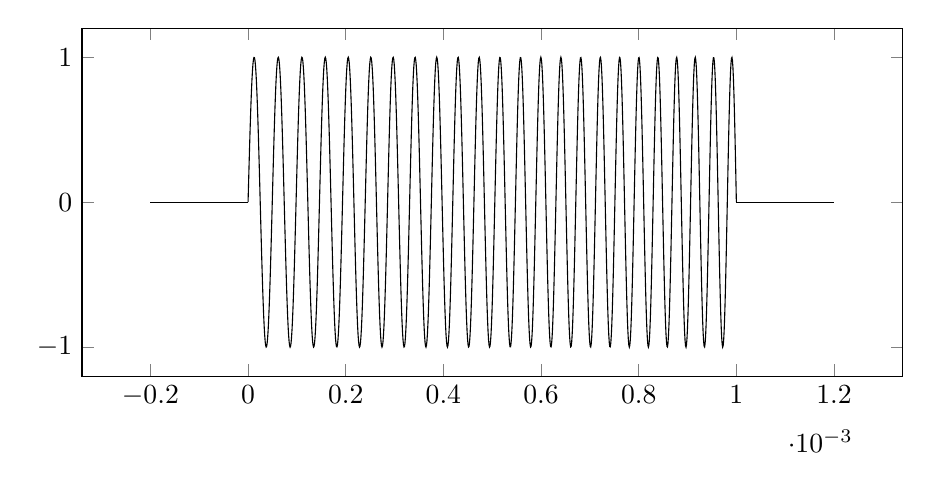
\begin{tikzpicture}
    \begin{axis}[width=12cm,height=6cm]
      \addplot[domain=-.0002:0,samples=10]{0};
      \addplot[domain=0:0.001,samples=1000]{sin((2*180*((27000 - 20000)/(2*0.001)*x*x + 20000*x)))};
      \addplot[domain=0.001:0.0012,samples=10]{0};
    \end{axis}
  \end{tikzpicture}
  \label{fig:chirp}
  \caption{Chirp signal with $\phi=0$, $A=1$, $f_0=\SI{20}{\kilo\hertz}$, $f_1=\SI{27}{\kilo\hertz}$, and $T=\SI{1}{\milli\second}$}
\end{figure}

This is the waveform we will be emitting from the ultrasonic sensors. The benefit is that it can be high power and still allow the receiver to determine precisely where in the waveform it is listening. One method for doing this is to take the discrete short time Fourier transform, which will show us how the power at various frequencies changes over time. By applying the FFT at a particular instant during the chirp, we can determine the position in time within the chirp of the current FFT. For instance, in the signal above if we apply and FFT at time $t_n=1.0$ and discover high power at frequency $f=\SI{22}{\kilo\hertz}$, we know that the chirp began at time $t_0 = t_n - \tfrac{f - f_0}{f_1 - f_0}T = 1.0 - \tfrac{22-20}{27-20}0.001 = 0.99857$. Another simpler strategy is to slide the waveform you expect to hear across samples of recorded raw input and check for the point of highest correlation. In other words, slide the waveform in figure \ref{fig:chirp} and match it to the received signal. Both of these techniques are used in practice, and we are considering both in our implementation. \cmmnt{what are the pros and cons}

Our beacon system relies on accurately knowing the distance to a beacon, and therefore knowing exactly when the start of the signal left the transmitter and when the start of the signal arrived at the receiver. Figure \ref{fig:rx_tx_timing} shows the sources of delay we are accounting for, and we describe our methodology for measuring these delays in the \nameref{experiments} section.

\begin{figure}
  \centering
  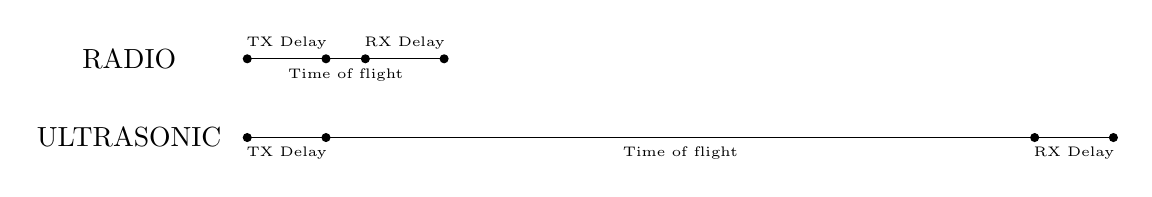
\begin{tikzpicture}
    % timeline for ultrasonic
    \draw (-1.5, 0) node {ULTRASONIC};
    \filldraw (0,0) circle (0.05);
    \draw (0.5, -0.2) node {\tiny TX Delay};
    \draw (0,0) -- (1,0);
    \filldraw (1,0) circle (0.05);
    \draw (5.5, -0.2) node {\tiny Time of flight};
    \draw (1,0) -- (10,0);
    \filldraw (10,0) circle (0.05);
    \draw (10.5, -0.2) node {\tiny RX Delay};
    \draw (10,0) -- (11,0);
    \filldraw (11,0) circle (0.05);

    % timeline for radio
    \draw (-1.5, 1) node {RADIO};
    \filldraw (0,1) circle (0.05);
    \draw (0.5, 1.2) node {\tiny TX Delay};
    \draw (0,1) -- (1,1);
    \filldraw (1,1) circle (0.05);
    \draw (1.25, 0.8) node {\tiny Time of flight};
    \draw (1,1) -- (1.5,1);
    \filldraw (1.5,1) circle (0.05);
    \draw (2.0, 1.2) node {\tiny RX Delay};
    \draw (1.5,1) -- (2.5,1);
    \filldraw (2.5,1) circle (0.05);
  \end{tikzpicture}
  \label{fig:rx_tx_timing}
  \caption{Timing of radio and ultrasonic signals}
\end{figure}

\textbf{Path Loss} \\
We calculate the free space path loss (FSPL) at the farthest distance from the beacons. For this calculation, we assume the worst case where the beacon is on the other side of the field, which is $\SI{16.5}{\meter}$ away.
$$ \text{FSPL} = 20\log_{10}\Bigg(\frac{4\pi Rf^2}{c^2}\Bigg) = 20\log_{10}\Bigg(\frac{4\pi*16.5*\SI{433e6}{\hertz}}{\SI{3e8}{\meter\per\second}}\Bigg) = 49.521 $$
% TODO: explain the parts we know in detail, like the proposed beacon protocol

% TODO: Setup appendix for things like the survey

\section{Conclusion} \label{conclusion}

\section{Appendix}
\subsection{Appendix A}\label{appendix:survey}

  Survey Responses

  \begin{figure}[H]
    \centering
    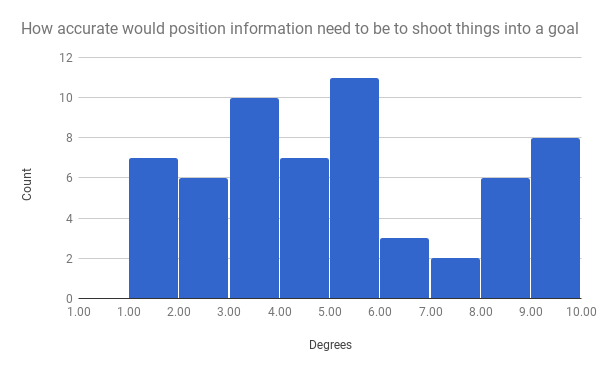
\includegraphics[width=1\linewidth]{./images/survey_angle.png}
    \label{fig:survey_angle}
  \end{figure}

  \begin{figure}[H]
    \centering
    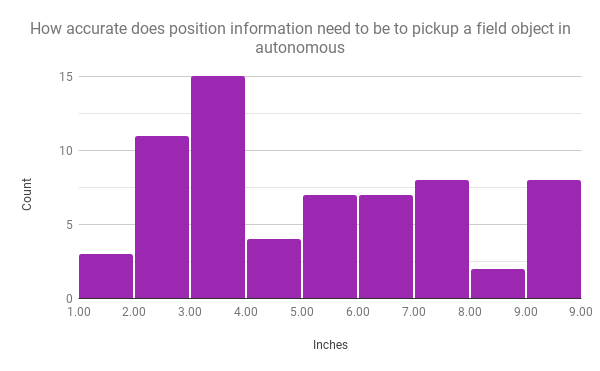
\includegraphics[width=1\linewidth]{./images/survey_position.png}
    \label{fig:survey_position}
  \end{figure}

  \begin{figure}[H]
    \centering
    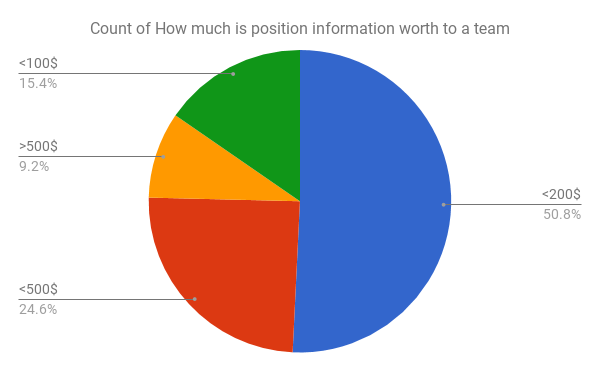
\includegraphics[width=1\linewidth]{./images/survey_worth.png}
    \label{fig:survey_worth}
  \end{figure}

\subsection{Appendix B}\label{appendix:rf-rx-tx}

\begin{table}[H]
  \begin{tabular}{|l|l|l|l|l|}
    \hline
    Measured Distance (m) & \multicolumn{3}{l|}{Measured Total Time (\mu s)} & Average Delay (\mu s) \\
    \hline
    0.0630 & 45.44 & 42.80 & 34.48 & 40.90646 \\
    0.1425 & 52.72 & 50.48 & 52.09 & 51.76286 \\
    0.1505 & 64.16 & 63.36 & 60.24 & 62.58616 \\
    0.2210 & 40.33 & 36.79 & 36.40 & 37.83926 \\
    0.2415 & 49.52 & 45.76 & 43.92 & 46.39919 \\
    0.2460 & 47.47 & 53.84 & 44.71 & 48.67251 \\
    0.2965 & 34.36 & 34.00 & 43.76 & 37.37234 \\
    0.3085 & 79.36 & 62.16 & 59.52 & 67.01230 \\
    0.3390 & 39.92 & 57.27 & 38.96 & 45.38220 \\
    0.3770 & 41.75 & 40.75 & 45.53 & 42.67541 \\
    0.3600 & 38.40 & 38.40 & 37.68 & 38.15880 \\
    0.0070 & 35.60 & 36.08 & 34.32 & 35.33331 \\
    \hline
    \multicolumn{4}{|l}{Overall Average Delay (\mu s)} & 46.175 \\
    \hline
  \end{tabular}
  \caption{The time of flight of radio over tens of centimeters is insignificant compared to the delay within the transmitter and receiver.}
  \label{table:rf-rx-tx}
\end{table}

\bibliographystyle{plain}
\bibliography{phil-mqp}
\end{document}
